%% This is file `elsarticle-template-1-num.tex',
%%
%% Copyright 2009 Elsevier Ltd
%%
%% This file is part of the 'Elsarticle Bundle'.
%% ---------------------------------------------
%%
%% It may be distributed under the conditions of the LaTeX Project Public
%% License, either version 1.2 of this license or (at your option) any
%% later version.  The latest version of this license is in
%%    http://www.latex-project.org/lppl.txt
%% and version 1.2 or later is part of all distributions of LaTeX
%% version 1999/12/01 or later.
%%
%% Template article for Elsevier's document class `elsarticle'
%% with numbered style bibliographic references
%%
%% $Id: elsarticle-template-1-num.tex 149 2009-10-08 05:01:15Z rishi $
%% $URL: http://lenova.river-valley.com/svn/elsbst/trunk/elsarticle-template-1-num.tex $
%%
\documentclass[preprint,12pt]{elsarticle}

%% Use the option review to obtain double line spacing
%% \documentclass[preprint,review,12pt]{elsarticle}

%% Use the options 1p,twocolumn; 3p; 3p,twocolumn; 5p; or 5p,twocolumn
%% for a journal layout:
%% \documentclass[final,1p,times]{elsarticle}
%% \documentclass[final,1p,times,twocolumn]{elsarticle}
%% \documentclass[final,3p,times]{elsarticle}
%% \documentclass[final,3p,times,twocolumn]{elsarticle}
%% \documentclass[final,5p,times]{elsarticle}
%% \documentclass[final,5p,times,twocolumn]{elsarticle}

%% The graphicx package provides the includegraphics command.
\usepackage{graphicx}
%% The amssymb package provides various useful mathematical symbols
\usepackage{amssymb}
%% The amsthm package provides extended theorem environments
%% \usepackage{amsthm}
%% following packages allows to write algorithms as pseudocode
\usepackage{amsmath}
\usepackage{algorithmicx}
\usepackage{algorithm}
\usepackage{algpseudocode}
\algnewcommand\algorithmicinput{\textbf{INPUT:}}
\algnewcommand\INPUT{\item[\algorithmicinput]}
\algnewcommand\algorithmicoutput{\textbf{OUTPUT:}}
\algnewcommand\OUTPUT{\item[\algorithmicoutput]}

%% The lineno packages adds line numbers. Start line numbering with
%% \begin{linenumbers}, end it with \end{linenumbers}. Or switch it on
%% for the whole article with \linenumbers after \end{frontmatter}.
\usepackage{lineno}

%% natbib.sty is loaded by default. However, natbib options can be
%% provided with \biboptions{...} command. Following options are
%% valid:

%%   round  -  round parentheses are used (default)
%%   square -  square brackets are used   [option]
%%   curly  -  curly braces are used      {option}
%%   angle  -  angle brackets are used    <option>
%%   semicolon  -  multiple citations separated by semi-colon
%%   colon  - same as semicolon, an earlier confusion
%%   comma  -  separated by comma
%%   numbers-  selects numerical citations
%%   super  -  numerical citations as superscripts
%%   sort   -  sorts multiple citations according to order in ref. list
%%   sort&compress   -  like sort, but also compresses numerical citations
%%   compress - compresses without sorting
%%
%% \biboptions{comma,round}

% \biboptions{}

% TODO notes, http://www.howtotex.com/packages/marking-things-to-do-with-todonotes/
\usepackage{todonotes}
% math tools (ceiling signs, see: http://tex.stackexchange.com/questions/42271/floor-and-ceiling-functions)
\usepackage{mathtools}
\DeclarePairedDelimiter{\ceil}{\lceil}{\rceil}

% new commands
\newcommand{\mtrx}[1]{\mathbf{#1}}

\journal{Advances in Engineering Software}

\begin{document}

\begin{frontmatter}

%% Title, authors and addresses

% consider omission of word 'Used' in title
\title{Singular Value Decomposition Used for Compression of Results from the Finite Element Method}

%% use the tnoteref command within \title for footnotes;
%% use the tnotetext command for the associated footnote;
%% use the fnref command within \author or \address for footnotes;
%% use the fntext command for the associated footnote;
%% use the corref command within \author for corresponding author footnotes;
%% use the cortext command for the associated footnote;
%% use the ead command for the email address,
%% and the form \ead[url] for the home page:
%%
%% \title{Title\tnoteref{label1}}
%% \tnotetext[label1]{}
%% \author{Name\corref{cor1}\fnref{label2}}
%% \ead{email address}
%% \ead[url]{home page}
%% \fntext[label2]{}
%% \cortext[cor1]{}
%% \address{Address\fnref{label3}}
%% \fntext[label3]{}


%% use optional labels to link authors explicitly to addresses:
%% \author[label1,label2]{<author name>}
%% \address[label1]{<address>}
%% \address[label2]{<address>}

\author{}
\address{Prague, Czech Republic}

\begin{abstract}
%% Text of abstract should have three parts: Motivation. This paper. Summary.
Amount of data produced by complex finite element analysis can be enormous and typical personal computer is not capable to store, process and visualize the results in reasonable time. Singular Value Decomposition (SVD) is well known factorization method that provides rich information about matrix systems. One of its many applications is image compression where it can significantly reduce size of data representing image while preserving quality of image appearance.
\newline
This paper describes application of SVD to the compression of results from finite element solvers. Although the idea of image compression method is inspiration for this research work, the SVD compression algorithm used for compression of images can not be directly used upon FEM results. Differences and implementation challenges are discussed in the text. Quality of approximation is more important in scientific field then in computer graphics where the main deciding factor is the human perception of the resulting image. Error estimation methods used during compression of finite element results are presented in the text. The focus is also on the algorithm performance. SVD is very computational intensive method. Various optimization techniques, e.g. Randomized SVD, are described in the text.
\newline
The results of the method are presented on various finite element analyses. The compression factor depends on the nature of input data. However, for common cases that were investigated the method achieves to lower the memory consumption at least to 10\% of the original size with negligible approximation error. In some cases the compression ratio can be even better. The important property of the method is ability to control the quality of compression.

\end{abstract}

\begin{keyword}
%% keywords here, in the form: keyword \sep keyword
Finite Element Method \sep FEM \sep Compression \sep Singular Value Decomposition \sep SVD \sep Principal Component Analysis \sep Data Visualization

% TODO: keyword PCA: vymazat nebo uvest v textu

%% MSC codes here, in the form: \MSC code \sep code
%% or \MSC[2008] code \sep code (2000 is the default)

\end{keyword}

\end{frontmatter}

%%
%% Start line numbering here if you want
%%
%\linenumbers

%% main text

% State of the art in FEM data compression
\section{Introduction}
\label{sec:introduction}

% Introduction to field of FEM results post-processing. Description of all terms used.

The effort to reduce size of resulting data from complex finite element analyses to accelerate (or even make possible) post-processing using common personal computer is not new.
\todo[inline]{State of the art. Add references to work in this field.}
In \cite{Benes2015} is presented one possible direction for research in this area -- the replacement of discrete data produced by finite element solver by simple continuous functions. These approximation functions can be then described be low number of parameters. The focus is on \textit{geometry}. The main goal is to find the areas in domain where the output discrete function has predictable development and can be easily replaced by e.g. linear continuous function. Although this approach has great results for some class of functions it is not applicable to problem in general. For some special cases, such as functions with discontinuities, the method has poor results because approximation error is too high and -- what is more important -- it can not be controlled in advance.

In this study the purely \textit{algebraic} approach is applied.

\todo[inline]{Describe alternative methods for compression: e.g. discrete 9/7 bi-orthogonal wavelet transform, discrete cosine transform, Karhunen-Loeve transform, and combinations of these}

\subsection{Related work / State of the art}

% Mathematical background
\section{Mathematical background}
\label{sec:math}

Singular value decomposition is based on a theorem from linear algebra which says that a rectangular matrix $\mtrx{A} \in \mathbb{R}^{m \times n}$ can be decomposed into the product of three matrices - an orthogonal matrix $\mtrx{U} \in \mathbb{R}^{m \times m}$, a diagonal
matrix $\mtrx{S} \in \mathbb{R}^{m \times n}$, and the transpose of an orthogonal matrix $\mtrx{V} \in \mathbb{R}^{n \times n}$:

\begin{equation}
\mtrx{A} = \mtrx{U} \mtrx{S} \mtrx{V}^\mathsf{T},
\label{eq:svd-def}
\end{equation}

\noindent
where $\mtrx{U^\mathsf{T}U} = \mtrx{I}$, $\mtrx{V^\mathsf{T}V} = \mtrx{I}$. The columns of $\mtrx{U}$ are orthonormal eigenvectors of $\mtrx{AA^\mathsf{T}}$, which are called the left singular vectors. The columns of $\mtrx{V}$ are orthonormal eigenvectors of $\mtrx{A^\mathsf{T}A}$ called the right singular vectors. $\mtrx{S}$ (sometimes referred to as $\mtrx{\Sigma}$) is a diagonal matrix containing singular values in descending order, which are at the same time the nonzero square roots of the eigenvalues of $\mtrx{AA^\mathsf{T}}$ and $\mtrx{A^\mathsf{T}A}$.

SVD can be seen as a method for transforming correlated variables into a set of uncorrelated ones. At the same time, SVD is a method for ordering the dimensions based on variation and identifying the dimension with the largest variation. Once this dimension is identified, it is possible to find the best approximation of the original data points using fewer dimensions. Hence, SVD can be seen as a method for data reduction/compression.

\subsection{SVD compression}

This is the basic idea behind SVD: taking a high dimensional, highly variable set of data points and reducing it to a lower dimensional space that exposes the substructure of the original data more clearly and orders it from the largest variation to the least. What makes SVD practical for data compression applications is that variation below a particular threshold can be simply ignored to massively reduce data with assurance that the main relationships of interest have been preserved.

The objective of a compression algorithm is to reduce amount of data representing FEM results and also the ability to reconstruct original data from its smaller representation. This saves storage capacity and also accelerates the data transfer between computers as the analysis itself and the post-processing of results is sometimes done on different workstations.

A compression method can be lossy or lossless. Lossless methods are able to fully reconstruct original data. Lossy methods, on the other hand, produce only approximations of original data.

SVD is used in this paper as a part of the compression algorithm. The SVD method applied to arbitrary matrix produces decomposition that consists of corresponding singular values and singular vectors. This process is fully reversible (with the assumption that the numerical errors are negligible). The original matrix can be reconstructed by the multiplication of decomposed parts. However, the compression algorithm is based on modification of decomposition to create low-rank approximation matrix. The reconstructed matrix slightly differs from the original matrix and algorithm therefore performs lossy compression.

\subsection{Low-rank approximation matrix}

From the definition of SVD in (\ref{eq:svd-def}) and from the properties of SVD, the fact follows that a matrix can be represented in the form of its SVD components as a sum of $k$ rank-1 matrices

\begin{equation}
\mtrx{A}=\sum_{i=1}^{k} s_{i}\mathbf{u}_{i}\mathbf{v}_{i}^{\mathsf{T}},
\label{eq:svd-expansion}
\end{equation}

\noindent
where $s_i$ is the $i$-th singular value of matrix $\mtrx{A}$, $\mathbf{u}_i$ and $\mathbf{v}_i$ are corresponding singular vectors of matrix $\mtrx{A}$, and $k = \mathrm{min}(m, n)$. Considering the fact that singular values are ordered $s_{1} \geq s_{2} \geq s_{3} \geq ... \geq s_{k}$, the above formula implies that the first term of the sum would have the highest contribution and the last term would have the lowest contribution to matrix~$\mtrx{A}$. Therefore, if we take only first $r$ members of the above summation we get an approximation matrix

\begin{equation}
\mtrx{A'}=\sum_{i=1}^{r} s_{i}\mathbf{u}_{i}\mathbf{v}_{i}^{\mathsf{T}}.
\label{eq:svd-approx-expansion}
\end{equation}

Quality of approximation depends on the magnitude of the singular values omitted from the approximation formula, namely $s_{r+1} ...  s_{k}$. The compression algorithm is based on an assumption that the first singular value is order-of-magnitude higher than singular values at the end of the decomposition sequence. In special cases, when $r=k$, or $s_{i}=0$ for all $i > r$, the omitted singular values do not contribute to the sum and the compression is therefore lossless. In other cases, approximation error has to be calculated and taken into account to avoid loss of important details in data.

The main goal of the compression algorithm is to find a compromise between low approximation error and high compression ratio $c$ which is calculated using the formula

\begin{equation}
c=\frac{r(m+n+1)}{m n},
\label{eq:cr-def}
\end{equation}

\noindent
where $m$ is the number of rows and $n$ is the number of columns of matrix $\mtrx{A}$. Explanation of the compression ratio formula is best done using Figure~\ref{fig:lowrank_svd}. Light color represents the part of matrix decomposition that is to be stored in the output file as a low-rank approximation of the input.

\begin{figure}[H]
\centering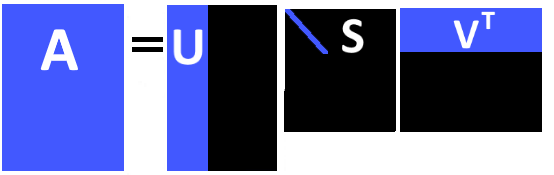
\includegraphics[width=0.7\textwidth]{figures/low_rank_decomposition_diagram}
\caption{Decomposition of input matrix $\mtrx{A}$ into diagonal matrix of singular values $\mtrx{S}$ and matrices of left and right singular vectors. Light color illustrates low-rank approximation.}
\label{fig:lowrank_svd}
\end{figure}

\subsection{Error estimation}
\label{sec:error}

Low-rank approximation matrix method that is described in this paper is a lossy compression technique. Several error metrics are used to control the quality of results.

\begin{itemize}

\item \textbf{Mean Square Error}
\begin{equation}
\mathit{MSE}=\frac{1}{m n} \sum_{i=1}^{m} \sum_{j=1}^{n} (a_{ij} - a'_{ij})^{2},
\label{eq:mse-def}
\end{equation}

\noindent
where $a_{ij}$ represents an element of the original matrix and $a'_{ij}$ represents an element of the
reconstructed matrix of dimension $m \times n$.

\item \textbf{Rooted Mean Square Deviation}
\begin{equation}
\mathit{RMSD} = \sqrt{\mathit{MSE}}.
\label{eq:rmsd-def}
\end{equation}

\item \textbf{Normalized Rooted Mean Square Deviation}
\begin{equation}
\mathit{NRMSD} = \frac{\mathit{RMSD}}{X_{max}-X_{min}}=\frac{\sqrt{\mathit{MSE}}}{X_{max}-X_{min}},
\label{eq:nrmsd-def}
\end{equation}

\noindent
where $X_{min}$ and $X_{max}$ are elements of input matrix $\mtrx{A}$ with minimum and maximum value, respectively. This error metric is able to measure and compare errors in datasets with different scales. Therefore, it is the main parameter that is used to control the quality of compression in the algorithm presented in this paper.

\item \textbf{Peak Signal to Noise Ratio}

$\mathit{PSNR}$ is most commonly used to measure the quality of reconstruction of lossy compression methods (e.g. image compression). The signal in this case is the original data, and the noise is the error introduced by compression. $\mathit{PSNR}$ is an approximation to human perception of reconstruction quality. This metric is not so important in area of FEM analyses, where the human perception of visualizations is not as important as the exact mathematical accuracy of approximations. The reason to include $\mathit{PSNR}$ in results is in particular to allow comparison with other image-related compression methods. $\mathit{PSNR}$ is usually expressed in terms of the logarithmic decibel scale (dB)

\begin{eqnarray}
\mathit{PSNR} &=& 10\log_{10}\frac{(X_{max}-X_{min})^{2}}{\mathit{MSE}} =
\\
&=& 20\log_{10}\frac{X_{max}-X_{min}}{\sqrt{\mathit{MSE}}}=20\log_{10}\frac{1}{\mathit{NRMSD}} = \nonumber
\\
&=& -20\log_{10}\mathit{NRMSD}. \nonumber
\label{eq:psnr-def}
\end{eqnarray}

\item \textbf{Normalized Maximum Error}
\begin{equation}
\mathit{NME} = \frac{\lVert \mtrx{A} - \mtrx{A'} \lVert_{\max}}{X_{max}-X_{min}} = \frac{\max\limits_{ij}(a_{ij} - a'_{ij})}{X_{max}-X_{min}}.
\label{eq:nme-def}
\end{equation}

\end{itemize}

\subsection{Randomized SVD}

The exact SVD of a $m \times n$ matrix has computational complexity \newline $\mathrm{O}(\mathrm{min}(mn^2, m^2n))$ using the "big-O" notation. When applied on large data sets it tends to be very time-consuming. In \cite{Candes2011, Woolfe2008, Martinsson2011, Szlam2014}, there are described randomized methods for constructing approximate matrix factorizations which offer significant speedups over classical methods.

% TODO: remove the 4 citations; pridat obecne kecy, v jakych oblastech se toto da a neda pouzit - tutorial page 5
% https://stats.stackexchange.com/questions/159325/what-fast-algorithms-exist-for-computing-truncated-svd - ruzne pristupy k vypoctu SVD

The particular implementation of the randomized decomposition is based on the algorithm described in \cite{Halko2011}. The authors proposed an algorithm for efficient computation of low-rank approximation to a given matrix. The algorithm can be split into two main computational stages.

The first stage is to construct a low-dimensional subspace that captures the action of the matrix. To be more formal, this stage is to compute an approximate basis for the range of the input matrix $\mtrx{A}$. This basis matrix $\mtrx{Q}$ is required to have orthonormal columns and

\begin{equation}
\mtrx{A} \approx \mtrx{Q} \mtrx{Q}^{\mathsf{T}} \mtrx{A}.
\end{equation}

\noindent
Matrix $\mtrx{Q}$ is desired to contain as few columns as possible while producing accurate approximation of matrix $\mtrx{A}$ at the same time.

The second stage is to use $\mtrx{Q}$ to obtain approximate SVD factorization of $\mtrx{A}$. This can be achieved using simple deterministic steps:

\begin{enumerate}
\item Construct $\mtrx{B} = \mtrx{Q}^{\mathsf{T}} \mtrx{A}$.
\item Compute an exact SVD of the small matrix: $\mtrx{B}=\mtrx{W}\mtrx{\widetilde{S}}\mtrx{\widetilde{V}}^{\mathsf{T}}$.
\item Set $\mtrx{\widetilde{U}}=\mtrx{Q}\mtrx{W}$.
\end{enumerate}

The main challenge is therefore to efficiently construct $r$ orthonormal vectors forming the matrix $\mtrx{Q}$ that (nearly) span the range of $\mtrx{A}$; $r$ is the desired rank of approximation and is supposed to be substantially less then both dimensions of $\mtrx{A}$. After that an SVD that closely approximates $\mtrx{A}$ can be constructed (closely in the sense that the spectral norm of the difference between $\mtrx{A}$ and the approximation to $\mtrx{A}$ is small relative to the spectral norm of $\mtrx{A}$).

In order to estimate the range of matrix $\mtrx{A}$, it is applied to a collection of $r$ random vectors. The result of applying $\mtrx{A}$ to any vector is a vector in the range of $\mtrx{A}$, and if the matrix is applied to $r$ random vectors, the results will nearly span the range of $\mtrx{A}$ with extremely high probability. Mathematical proofs given in \cite{Halko2011} and \cite{Witten2015} show that the probability of missing a substantial part of the range of $\mtrx{A}$ is negligible if the vectors to which we apply $\mtrx{A}$ are sufficiently random (i.e. entries of these vectors are independent and identically distributed).

Therefore, the matrix $\mtrx{A}$ is applied to a random Gaussian matrix $\mtrx{\Omega}$ that contains $r$ columns with random normally distributed entries yielding the matrix $\mtrx{Y} = \mtrx{A} \mtrx{\Omega}$. Applying the Gram-Schmidt process (or any other method for constructing QR decomposition) produces the decomposition $\mtrx{Y}=\mtrx{Q}\mtrx{R}$, where columns of $\mtrx{Q}$ are an orthonormal basis for the range of $\mtrx{Y}$, and since columns of $\mtrx{Y}$ nearly span the range of $\mtrx{A}$, $\mtrx{Q}$ is an orthonormal basis for the approximate range of $\mtrx{A}$.

$\mtrx{A}$ is then decomposed as
\begin{equation}
\mtrx{A} \approx \mtrx{Q}\mtrx{Q}^{\mathsf{T}}\mtrx{A} = \mtrx{Q}\mtrx{B} = \mtrx{Q}\mtrx{W}\mtrx{\widetilde{S}}\mtrx{\widetilde{V}}^{\mathsf{T}} = \mtrx{\widetilde{U}}\mtrx{\widetilde{S}}\mtrx{\widetilde{V}}^{\mathsf{T}}.
\end{equation}

\noindent
The algorithm produces matrices $\mtrx{\widetilde{U}}$ and $\mtrx{\widetilde{V}}$ with orthonormal columns being approximations of the left and the right singular vectors of matrix $\mtrx{A}$, and a nonnegative diagonal matrix $\mtrx{\widetilde{S}}$ that contains approximations of the first $r$ singular values of matrix $\mtrx{A}$. For a dense input matrix, randomized SVD algorithm requires $\mathrm{O}(mn \log{r})$ floating-point operations, substantially less than classical algorithms.

% TODO: last sentence put in new paragraph
% Error estimators: tutorial Page 12
% Power iterations: research-fb

% TODO: explain gain in operation complexity (see tutorial page 13)

% do answers napsat, ze jsme doplnili ty a ty odstavce, ale ze nehodlame vice vysvetlovat samotny randomized algoritmus, protoze jeho implementace neni predmetem paperu

% Description of FEM data compression algorithm
\section{Implementation}
\label{sec:implementation}

The objective of the compression algorithm is to reduce amount of data representing FEM results and also the ability to reconstruct original data from its smaller representation. This saves storage capacity and also accelerates data transfer between computers as the analysis itself and the post-processing of results is usually done on different work stations.

Compression method can be lossy or lossless based on quality of data reconstructed of its compressed representation. Lossless methods are able to fully reconstruct original data. Lossy methods on the other hand produce only approximations of original data. 

SVD is used as part of the compression algorithm. SVD method applied to arbitrary matrix produces decomposition that consist of corresponding singular values and singular vectors. This process is fully reversible (with the assumption that the numerical errors are negligible). The original matrix can be reconstructed by the multiplication of decomposed parts. However, the compression algorithm is based on modification of decomposition to create low-rank approximation matrix. The reconstructed matrix slightly differs from the original matrix and algorithm therefore does lossy compression.

SVD decomposition is applied on matrices. The first thing to do is therefore to assemble an input matrix. Results from the Finite element method are discrete values calculated in nodes or integration points. There are usually multiple fields in result data (e.g. displacements, stress, strain etc.) and each field can have multiple components (e.g. displacements can have $X$, $Y$ and $Z$ component). As non-linear analyses usually lead to multiple computation steps there are multiple sets of data per each field component. All data corresponding to a single field component form the input matrix $\mtrx{A}$ to the compression algorithm. Only single field component is considered to fill the input matrix $\mtrx{A}$. Results for different data components (even for the same field) can be independent from each other. There can also be order-of-magnitude difference between the components and the compression algorithm could potentially clear the important information in the weaker component. Another reason against merging of components is computational complexity. The smaller the matrix $\mtrx{A}$ is, the faster the decomposition algorithm performs.

Each row of matrix $\mtrx{A}$ corresponds to single time step and each column corresponds to a single node or integration point. Once the matrix $\mtrx{A}$ is built for a field component the compression algorithm can be applied on it. It is purely algebraic procedure, no information about geometry of the mesh is needed. 

% The compression algorithm is based on low-rank approximation matrix created from SVD decomposition. Results for time steps are not independent. They usually have some relation between them. List of singular values produced by the SVD method reveals the dependency between the singular vectors that form the orthogonal base of the matrix $\mtrx{A}$.

\subsection{Low-rank approximation matrix}

From the definition of SVD in (\ref{eq:svd-def}) and from the properties of SVD presented in section \ref{sec:math} follows the fact that a matrix can be represented in the form of its SVD components as a sum of rank-1 matrices in the form

\begin{equation}
\mtrx{A}=\mtrx{U_{1}}S_{1}\mtrx{V_{1}^{T}}+\mtrx{U_{2}}S_{2}\mtrx{V_{2}^{T}}+ ... +\mtrx{U_{n}}S_{n}\mtrx{V_{n}^{T}},
\label{eq:svd-expansion}
\end{equation}

\noindent
where $S_{i}$ is $i$-th singular value, $\mtrx{U_{i}}$ and $\mtrx{V_{i}}$ are corresponding singular vectors, and $n$ is the rank of matrix~$\mtrx{A}$. Considering the fact that singular values are ordered $S_{1} \geq S_{2} \geq S_{3} \geq ... \geq S_{n}$ the above formula implies that the first term would have the highest contribution and last term would have the lowest contribution to matrix~$\mtrx{A}$. Therefore, if we take only first $r$ members of the above summation we get an approximation matrix

\begin{equation}
\mtrx{A'}=\mtrx{U_{1}}S_{1}\mtrx{V_{1}^{T}}+\mtrx{U_{2}}S_{2}\mtrx{V_{2}^{T}}+ ... +\mtrx{U_{r}}S_{r}\mtrx{V_{r}^{T}}.
\label{eq:svd-approx-expansion}
\end{equation}

The quality of approximation depends on the magnitude of the singular values omitted from the approximation formula, namely $S_{r+1} ...  S_{n}$. The compression algorithm is based on assumption that the first singular value is order-of-magnitude higher than singular values at the end of the decomposition sequence. In special cases, when $r=n$, or $S_{i}=0$ for all $i \geq r$ the omitted singular values do not contribute to the sum and the compression is therefore lossless. In other cases, approximation error has to be calculated and taken into account to avoid loss of important details in data.

The main goal of the compression algorithm is to find a compromise between low approximation error and high compression ratio $CR$ which is calculated using the formula

\begin{equation}
CR=\frac{r(m+n+1)}{m n},
\label{eq:cr-def}
\end{equation}

\noindent
where $m$ and $n$ are dimensions of matrix $\mtrx{A}$. Explanation of the compression ratio formula is best done using Figure~\ref{fig:lowrank_svd}. Light color represents the part of matrix decomposition that is to be stored in the output file as a low-rank approximation of the input.

\begin{figure}[H]
\centering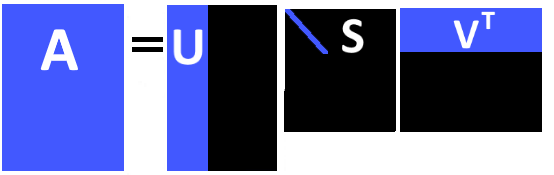
\includegraphics[width=0.7\textwidth]{figures/low_rank_decomposition_diagram}
\caption{Decomposition of input matrix $\mtrx{A}$ into diagonal matrix of singular values $\mtrx{\Sigma}$ and matrices of left and right singular vectors. Light color illustrates low-rank approximation.}
\label{fig:lowrank_svd}
\end{figure}

Let us assume that the matrix is not empty and has full-rank. Then from the formula above follows that if $r$ equals to the rank of matrix $\mtrx{A}$ the compression ratio is always higher than one. In other words the memory consumption of stored decomposition is bigger than the size of the original matrix. To make the compression algorithm applicable the parameter $r$ must conform to the condition

$$r<\frac{m n}{m+n+1}.$$

\noindent
Considering the usual shape of matrix containing FEM results this inequality is easily satisfiable even for the $r$ being close to the rank of the original matrix as in the typical case the number of nodes or integration-points is much higher than the number of analysis steps and therefore $m<<n$.

\subsection{Algorithm description}
Once the SVD decomposition is calculated the compression algorithm removes a certain number of singular values and corresponding singular vectors. The remaining singular values and vectors represent the compressed data. There are two strategies that influence the way how to get the number of singular values to be preserved -- resulting size and quality. Each strategy is assigned a control parameter that determines compression ratio or approximation error.

\paragraph{Compression ratio}
If the focus is only on the size of compressed data, the rank $r$ of the approximation matrix can be calculated by the formula

\begin{equation}
r=\ceil*{CR \times \frac{m n}{m+n+1}},
\end{equation}

\noindent
where $CR$ is the compression ratio, $0 \leq CR \leq 1$ ($0$ results in absolute compression while $1$ results in no compression).

\paragraph{Approximation error}
In the usual case the most important parameter to take into account is the approximation error. Algorithm is trying to minimize the compression ratio while at the same time ensuring that predefined limit of approximation error is not exceeded. To quantify the error the Mean squared error ($MSE$) metric is used. To be able to compare different data-sets having different scales the normalized version of $MSE$ is used - Normalized root-mean-square deviation ($NRMSD$). Both metrics are defined in section \ref{sec:error}.

But how can be the rank of approximation matrix effectively calculated from the desired approximation error? Here comes useful the interesting property of the singular values:

% TODO: Reference to source or further explanation needed. (prof. Marek?)

\begin{equation}
\sum_{i=1}^{m} \sum_{j=1}^{n} (\mtrx{A_{ij}})^{2} = \sum_{i=1}^{k}{\sigma_{i}^{2}},
\label{eq:elem-sqr-sigma-sqr}
\end{equation}

\noindent
where $k=min(m, n)$, i.e. the smallest of two dimensions of the matrix $\mtrx{M}$. The above formula states that the sum of squared elements of matrix $\mtrx{A}$ equals to the sum of squared singular values $\sigma_{i}$ of the same matrix $\mtrx{A}$.

Using formulas \eqref{eq:svd-expansion} and \eqref{eq:svd-approx-expansion} the equation \eqref{eq:elem-sqr-sigma-sqr} can be applied to the difference between original matrix $\mtrx{A}$ and approximation matrix $\mtrx{A'}$.

\begin{equation}
\sum_{i=1}^{m} \sum_{j=1}^{n} (\mtrx{A_{ij}} - \mtrx{A'_{ij}})^{2} = \sum_{i=r+1}^{k}{\sigma_{i}^{2}},
\end{equation}

\noindent
where the term on the right-hand side is the sum of squares of those singular values of the matrix $A$ that are going to be cut away by the compression algorithm. The equation can be rewritten using the definition of $MSE$ in \eqref{eq:mse-def} to

\begin{equation}
MSE \times m n = \sigma_{r+1}^{2} + \sigma_{r+2}^{2} + ... + \sigma_{k-1}^{2} + \sigma_{k}^2
\end{equation}

\noindent
and using \eqref{eq:nrmsd-def} further to

\begin{equation}
(NRMSD \times (X_{max}-X_{min}))^{2} \times m n = \sigma_{r+1}^{2} + \sigma_{r+2}^{2} + ... + \sigma_{k-1}^{2} + \sigma_{k}^2.
\end{equation}

Then $NRMSD$ can be used as a quality metric for the compression algorithm because normalization makes it usable for different datasets. Calculation of rank of the approximation matrix is depicted as pseudo-code in algorithm \ref{alg:rank-calculation}. Algorithm uses the following inequality to test whether the desired rank has been reached

\begin{equation}
e > \frac{\sqrt[]{\frac{\sigma_{r+1}^{2} + \sigma_{r+2}^{2} + ... + \sigma_{k-1}^{2} + \sigma_{k}^2}{m n}}}{X_{max}-X_{min}},
\end{equation}

\noindent
where $e$ is NRMSD used as an error limit that can not be exceeded to achieve reasonable quality of approximation.

\begin{algorithm}
  \caption{Calculation of rank for approximation matrix from maximum allowed error}\label{rankAlgorithm}
  \label{alg:rank-calculation}
  \begin{algorithmic}[1]
  	\INPUT maximum allowed error ($e$), array with singular values ($S$), element count ($c$), maximum element value ($x_{max}$), minimum element value ($x_{min}$)
    \OUTPUT rank of resulting matrix
    \Procedure{CalculateRank}{$e, S, c, x_{max}, x_{min}$}
      \State $MSE \gets 0$
      \State $NRMSD \gets 0$
      \State $rank \gets S.length$
      \While{$NRMSD < e$}\Comment{repeat until max error is reached}
        \State $MSE \gets MSE + S[rank]/c$ \Comment{calculate MSE for current rank}
        \State $NRMSD \gets \sqrt{MSE} / (x_{max} - x_{min})$ \Comment{normalize error}
        \State $rank \gets rank - 1$ \Comment{decrement rank for next loop}
      \EndWhile
      \State \textbf{return} $rank + 1$ \Comment{Add one to not exceed maximum allowed error}
    \EndProcedure
  \end{algorithmic}
\end{algorithm}

\subsection{Optimization}

% http://mathoverflow.net/questions/161252/what-is-the-time-complexity-of-truncated-svd

Time complexity of the exact SVD decomposition algorithm is $O(m^2n)$, where $m<n$. This theoretical algorithm complexity is confirmed by two benchmarks where the dependency of execution time on varying matrix dimension is shown. The results of the benchmarks are depicted in Figure \ref{fig:ExeTime_rows} and Figure \ref{fig:ExeTime_columns}. Several observations were made from the results:

\begin{itemize}
\item The algorithm is most efficient in cases where one dimension of the input matrix is very low compared to the other. However, this is almost always the case when compressing results from FEM -- number of time steps seldom exceeds hundreds.
\item Moreover, time steps can be split into smaller ranges and the algorithm can be applied on each range separately. This will improve performance and can also increase quality of compression if the key time steps on the range boundaries are carefully selected.
\item Randomized SVD algorithm has the same order of algorithmic complexity but yet can help to significantly reduce execution time.
\end{itemize}

Storage size of SVD decomposition itself can also be optimized. $\mtrx{\Sigma}$ being a diagonal matrix can be stored as single list of singular values $\sigma_{i}$ or can be even multiplied with the matrix of left singular vectors $\mtrx{U}$.

% main features for optimization: key time steps (time step span compression), Randomized SVD, Parallelization, Sparse matrix of details, prenasobeni U matice singularnimi cisly, trochu usetrim pamet, mohu pouzit vzorkovani...


% Results of compression method (images from postprocessor, tables with compression ratio and error)
\section{Results}
\label{sec:results}

\begin{figure}[ht]
\centering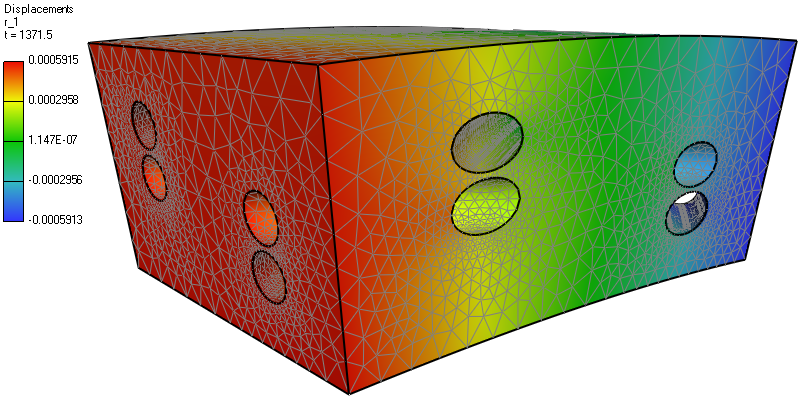
\includegraphics[width=\textwidth]{figures/temelin_screenshot}
\caption{Temelin nuclear power plant. Results visualization (Displacement field, X component).}
\label{fig:temelin:mesh}
\end{figure}

\begin{figure}[ht]
\centering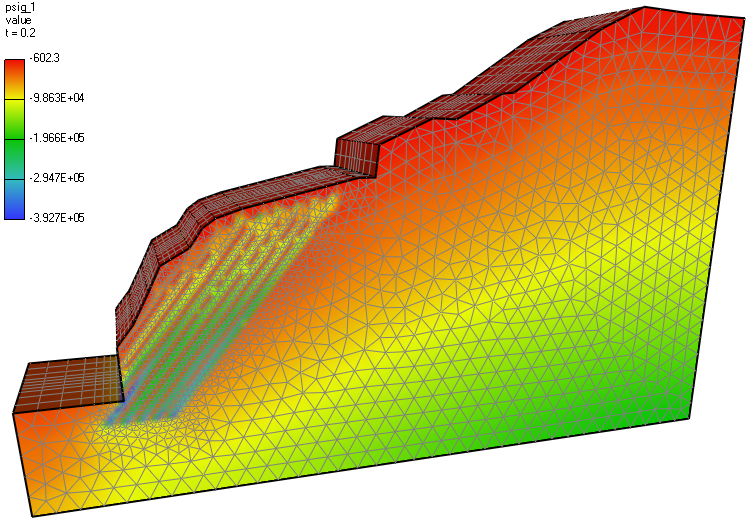
\includegraphics[width=\textwidth]{figures/chotkova_screenshot}
\caption{Chotkova geologic layers. Results visualization (Stress field, sigma XX component).}
\label{fig:chotkova:mesh}
\end{figure}

\begin{figure}[ht]
\centering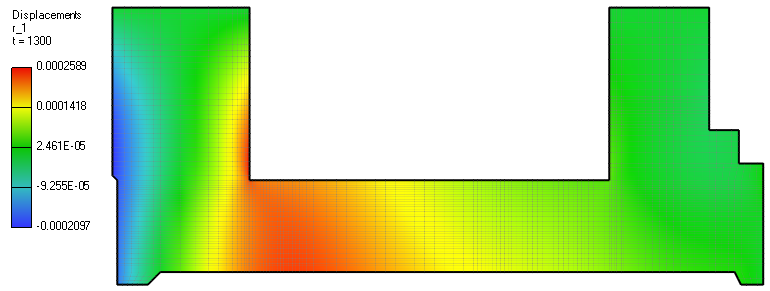
\includegraphics[width=\textwidth]{figures/mechaxisym_screenshot}
\caption{"Mechaxisym" model. Results visualization (Displacement field, X component).}
\label{fig:mechaxisym:mesh}
\end{figure}

\begin{figure}[ht]
\centering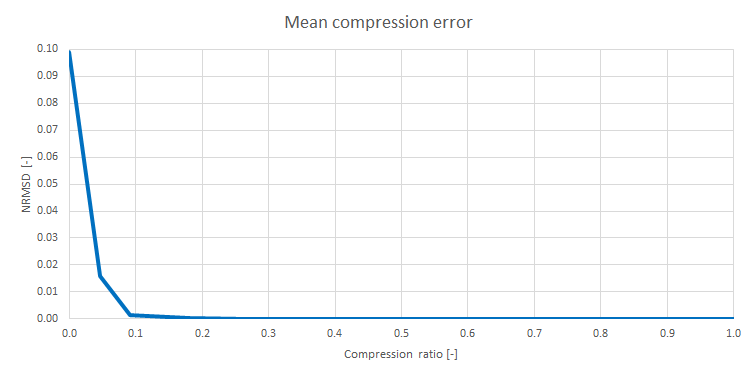
\includegraphics[width=\textwidth]{figures/chotkova_NRMSD}
\caption{Dependence of Normalized Rooted Mean Squared Deviation on Compression ratio for Chotkova project results.}
\label{fig:chotkova:NRMSD}
\end{figure}

\begin{figure}[ht]
\centering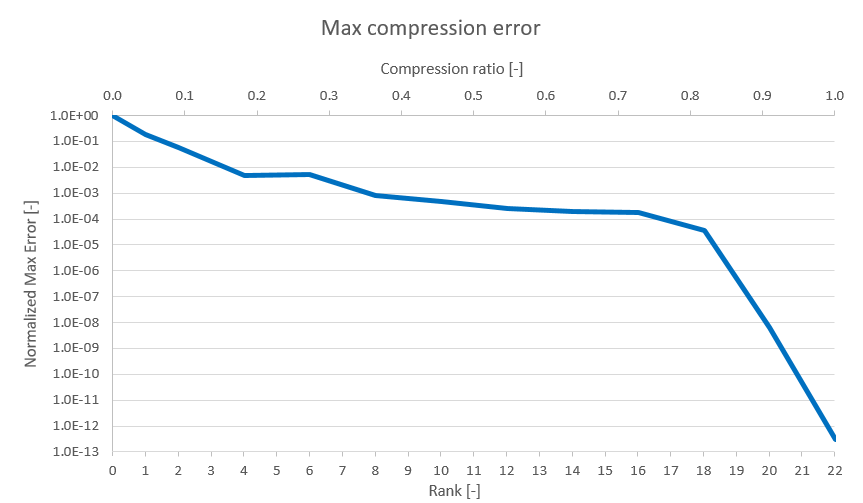
\includegraphics[width=\textwidth]{figures/chotkova_MaxError}
\caption{Dependence of Normalized Max Error on Compression ratio for Chotkova project results.}
\label{fig:chotkova:MaxError}
\end{figure}

\begin{figure}[ht]
\centering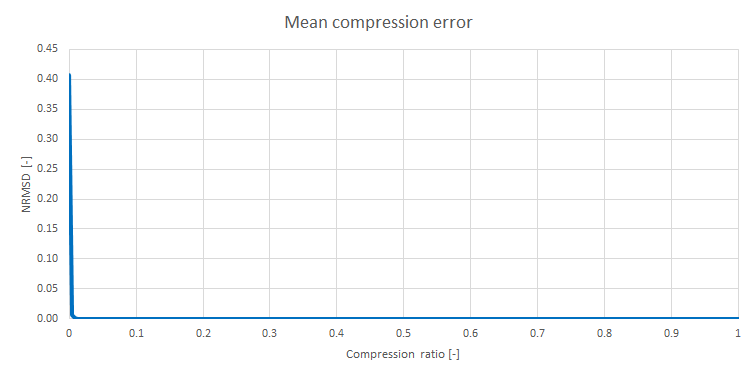
\includegraphics[width=\textwidth]{figures/mechaxisym_NRMSD}
\caption{Dependence of Normalized Rooted Mean Squared Deviation on Compression ratio for Mechaxisym project results.}
\label{fig:mechaxisym:NRMSD}
\end{figure}

\begin{figure}[ht]
\centering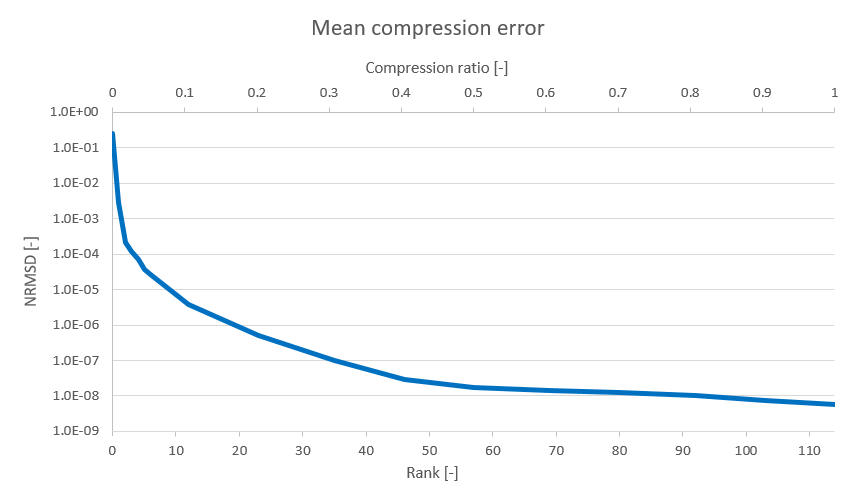
\includegraphics[width=\textwidth]{figures/temelin_NRMSD}
\caption{Dependence of Normalized Rooted Mean Squared Deviation on Compression ratio for Temelin project results.}
\label{fig:temelin:NRMSD}
\end{figure}

\begin{figure}[ht]
\centering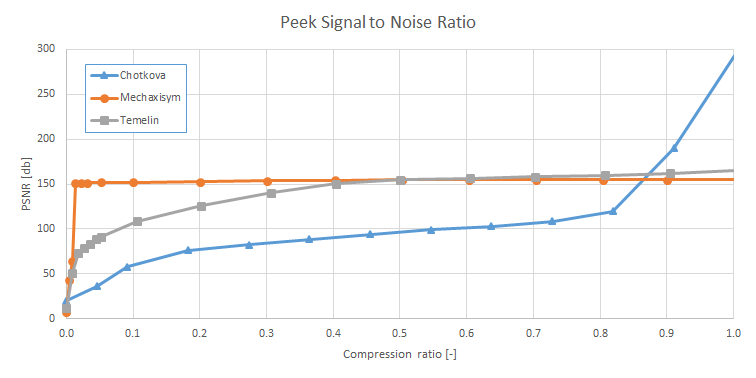
\includegraphics[width=\textwidth]{figures/PSNR}
\caption{Comparison of Peek signal to noise ratio value calculated for different decompositions.}
\label{fig:PSNR}
\end{figure}

\begin{figure}[ht]
\centering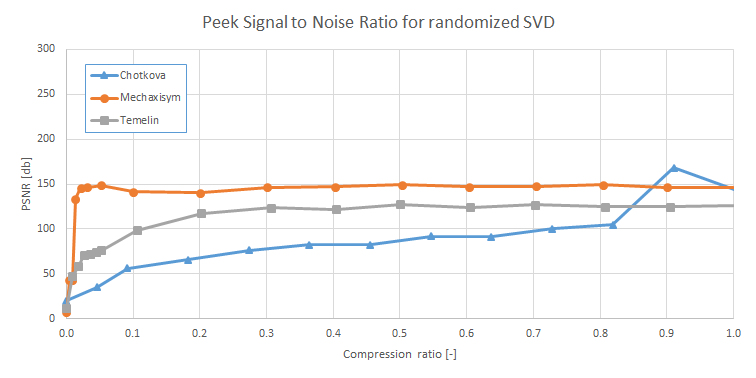
\includegraphics[width=\textwidth]{figures/PSNR_rand}
\caption{Comparison of Peek signal to noise ratio value for different randomized decompositions.}
\label{fig:PSNR_rand}
\end{figure}

\begin{figure}[ht]
\centering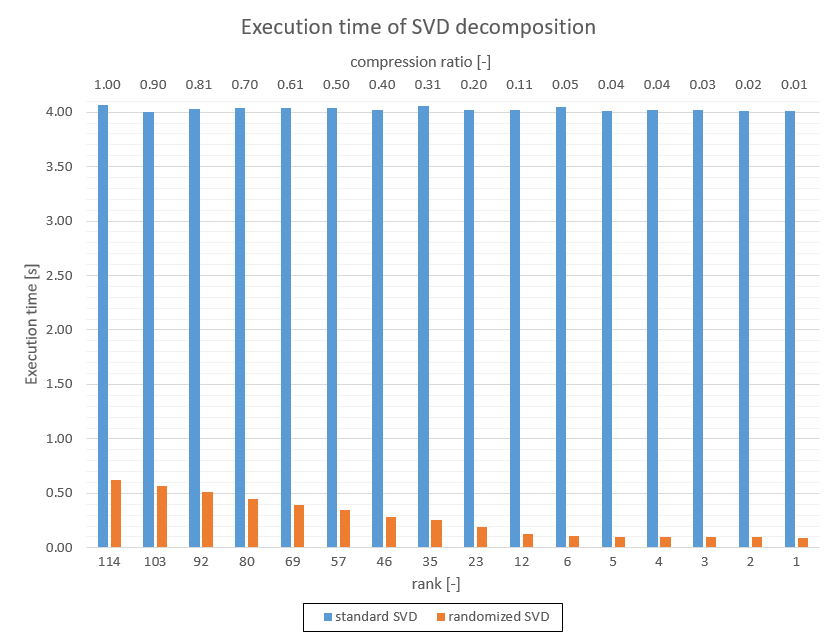
\includegraphics[width=\textwidth]{figures/temelin_ExecutionTime}
\caption{Variation of execution time of standard and randomized decompositions calculated for Temelin project results. Execution time of standard SVD is independent of target rank whereas execution time of randomized SVD decreases linearly with increasing target rank.}
\label{fig:temelin:ExeTime}
\end{figure}

\begin{figure}[ht]
\centering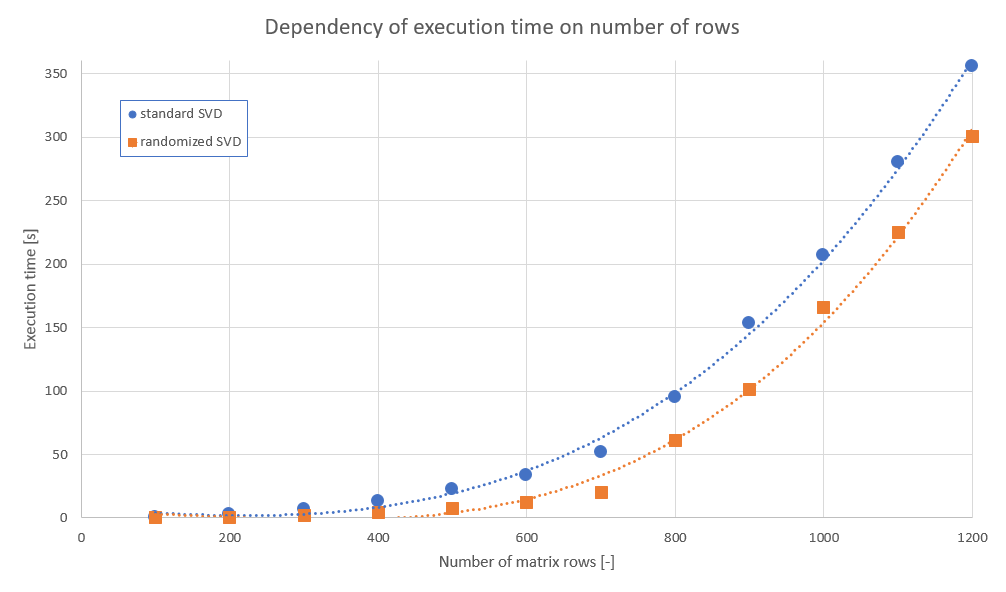
\includegraphics[width=\textwidth]{figures/executionTime_varyingRows}
\caption{Dependency of SVD execution time on number of rows of an input matrix.}
\label{fig:ExeTime_rows}
\end{figure}

\begin{figure}[ht]
\centering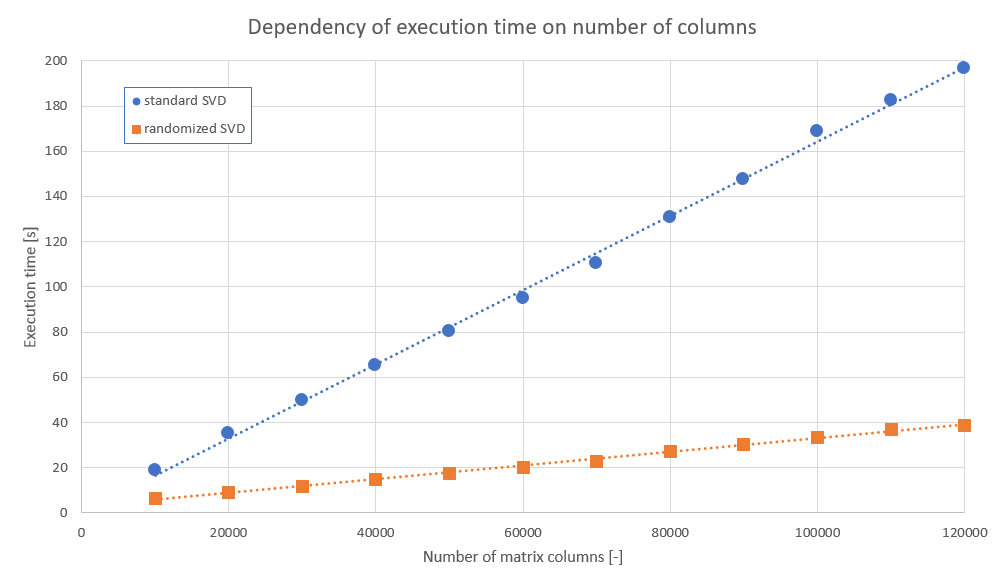
\includegraphics[width=\textwidth]{figures/executionTime_varyingColumns}
\caption{Dependency of SVD execution time on number of columns of an input matrix.}
\label{fig:ExeTime_columns}
\end{figure}

% Evaluation of results
\section{Conclusion}
\label{sec:conclusion}

The goal of this paper is to present the use of SVD in compression of results from the Finite Element Method. Implementation details of the compression algorithm have been provided, and the results of its application on real data have been presented. The implemented algorithm is able to compress arbitrary data using low-rank approximation matrices. When the maximum allowed error was set to $10^{-5}$, the compression ratio was at most 10\% for all tested results. In many cases compression ratio can be even better -- bellow 1\% of the original size. The important property of the compression algorithm is the fact that the approximation error can be set in advance and there is a guarantee that it will not be exceeded.

The main disadvantage is the computational complexity of the compression algorithm. SVD is a very time-consuming operation. However, this operation is performed only once after FEM analysis is finished and before the post-processing is started. Also, the randomized version of the decomposition algorithm is much faster and can be used if a slight increase of approximation error is tolerated.

Another complication is the necessity to use a special format to store compressed data in the form of matrix decompositions, and the post-processor must be updated to use this new format. Post-processor must perform matrix multiplication to get the original results. However, in a usual case the data for one analysis step are needed at a time, i.e. multiplication of a single row is enough. Detailed description of the post-processor implementation is beyond the scope of this paper.


% Acknowledgement
\section*{Acknowledgement}

%% The Appendices part is started with the command \appendix;
%% appendix sections are then done as normal sections
%% \appendix

%% \section{}
%% \label{}

%% References
%%
%% Following citation commands can be used in the body text:
%% Usage of \cite is as follows:
%%   \cite{key}          ==>>  [#]
%%   \cite[chap. 2]{key} ==>>  [#, chap. 2]
%%   \citet{key}         ==>>  Author [#]

%% References with bibTeX database:

\section*{References}

% TODO: doplnit informace k referencim
% TODO: upravit chyby ve formatovani referenci

\bibliographystyle{model1-num-names}
\bibliography{references.bib}

%% Authors are advised to submit their bibtex database files. They are
%% requested to list a bibtex style file in the manuscript if they do
%% not want to use model1-num-names.bst.

%% References without bibTeX database:

% \begin{thebibliography}{00}

%% \bibitem must have the following form:
%%   \bibitem{key}...
%%

% \bibitem{}

% \end{thebibliography}

% Test section to experiment with tex template
%\newpage
%\section*{Test section}

\textbf{Test section to experiment with tex template}
\linebreak

Reference to Section \ref{section:math}. Etiam congue sollicitudin diam non porttitor. Etiam turpis nulla, auctor a pretium non, luctus quis ipsum. Fusce pretium gravida libero non accumsan. Donec eget augue ut nulla placerat hendrerit ac ut mi. Phasellus euismod ornare mollis. Proin tempus fringilla ultricies. Donec pretium feugiat libero quis convallis. Nam interdum ante sed magna congue eu semper tellus sagittis. Curabitur eu augue elit.

Maecenas fermentum urna ac sapien tincidunt lobortis. Nunc feugiat faucibus varius. Ut sed purus nunc. Ut eget eros quis lectus mollis pharetra ut in tellus. Pellentesque ultricies velit sed orci pharetra et fermentum lacus imperdiet. Class aptent taciti sociosqu ad litora torquent per conubia nostra, per inceptos himenaeos. Suspendisse commodo ultrices mauris, condimentum hendrerit lorem condimentum et. Pellentesque urna augue, semper et rutrum ac, consequat id quam. Proin lacinia aliquet justo, ut suscipit massa commodo sit amet. Proin vehicula nibh nec mauris tempor interdum. Donec orci ante, tempor a viverra vel, volutpat sed orci.

Pellentesque habitant morbi tristique senectus et netus et malesuada fames ac turpis egestas. Pellentesque quis interdum velit. Nulla tincidunt sem quis nisi molestie nec hendrerit nulla interdum. Nunc at lectus at neque dapibus dapibus sit amet in massa. Nam ut nisl in diam consectetur dignissim. Sed lacinia diam id nunc suscipit vitae semper lorem semper. In vehicula velit at tortor fringilla elementum aliquam erat blandit. Donec pretium libero et neque vehicula blandit. Curabitur consequat interdum sem at ultrices. Sed at tincidunt metus. Etiam vulputate, lacus eget fermentum posuere, ante mi dignissim augue, et ultrices felis tortor sed nisl.

\begin{itemize}
\item Bullet point one
\item Bullet point two
\end{itemize}

\begin{enumerate}
\item Numbered list item one
\item Numbered list item two
\end{enumerate}

\subsection{Randomized SVD}

Quisque elit ipsum \cite{Benes15}, porttitor et imperdiet in, facilisis ac diam. Nunc facilisis interdum felis eget tincidunt. In condimentum fermentum leo, non consequat leo imperdiet pharetra. Fusce ac massa ipsum, vel convallis diam. Quisque eget turpis felis. Curabitur posuere, risus eu placerat porttitor, magna metus mollis ipsum, eu volutpat nisl erat ac justo. Nullam semper, mi at iaculis viverra, nunc velit iaculis nunc, eu tempor ligula eros in nulla. Aenean dapibus eleifend convallis. Cras ut libero tellus. Integer mollis eros eget risus malesuada fringilla mattis leo facilisis. Etiam interdum turpis eget odio ultricies sed convallis magna accumsan. Morbi in leo a mauris sollicitudin molestie at non nisl.

\begin{table}[ht]
\centering
\begin{tabular}{l l l}
\hline
\textbf{Treatments} & \textbf{Response 1} & \textbf{Response 2}\\
\hline
Treatment 1 & 0.0003262 & 0.562 \\
Treatment 2 & 0.0015681 & 0.910 \\
Treatment 3 & 0.0009271 & 0.296 \\
\hline
\end{tabular}
\caption{Table caption}
\end{table}

\subsection{Subsection Two}

Donec eget ligula venenatis est posuere eleifend in sit amet diam. Vestibulum sollicitudin mauris ac augue blandit ultricies. Nulla facilisi. Etiam ut turpis nunc. Praesent leo orci, tincidunt vitae feugiat eu, feugiat a massa. Duis mauris ipsum, tempor vel condimentum nec, suscipit non mi. Fusce quis urna dictum felis posuere sagittis ac sit amet erat. In in ultrices lectus. Nulla vitae ipsum lectus, a gravida erat. Etiam quam nisl, blandit ut porta in, accumsan a nibh. Phasellus sodales euismod dolor sit amet elementum. Phasellus varius placerat erat, nec gravida libero pellentesque id. Fusce nisi ante, euismod nec cursus at, suscipit a enim. Nulla facilisi.

\begin{figure}[ht]
\centering
\includegraphics[width=0.4\linewidth]{figures/placeholder}
\caption{Figure caption}
\end{figure}

Integer risus dui, condimentum et gravida vitae, adipiscing et enim. Aliquam erat volutpat. Pellentesque diam sapien, egestas eget gravida ut, tempor eu nulla. Vestibulum mollis pretium lacus eget venenatis. Fusce gravida nisl quis est molestie eu luctus ipsum pretium. Maecenas non eros lorem, vel adipiscing odio. Etiam dolor risus, mattis in pellentesque id, pellentesque eu nibh. Mauris nec ante at orci ultricies placerat ac non massa. Aenean imperdiet, ante eu sollicitudin vestibulum, dolor felis dapibus arcu, sit amet fermentum urna nibh sit amet mauris. Suspendisse adipiscing mollis dolor quis lobortis.

\begin{equation}
\label{eq:emc}
e = mc^2
\end{equation}

\end{document}
